\section{The GPU Evolution}
\subsection{History}
\begin{frame}{A Brief History}
  \begin{columns}
    \begin{column}{0.6\textwidth}
      \footnotesize
      \begin{timeline}
        \timelineitem{0}{1970s-1980s}{Software Rendering}{
          \begin{itemize}
              \scriptsize
            \item Everything done on CPU
            \item Frame rates: 1-10 FPS
            \item Wireframe graphics
          \end{itemize}
        }

        \timelineitem{1.2}{1990s}{Fixed-Function GPUs}{
          \begin{itemize}
              \scriptsize
            \item 3dfx Voodoo, NVIDIA Riva
            \item Hardware rasterization
            \item Fixed pipeline stages
          \end{itemize}
        }

        \timelineitem{1.2}{2000s}{Programmable Shaders}{
          \begin{itemize}
              \scriptsize
            \item DirectX 8.0, OpenGL
            \item Vertex \& Fragment shaders
            \item Creative freedom
          \end{itemize}
        }

        \timelineitem{1.2}{2010s+}{Unified Architecture}{
          \begin{itemize}
              \scriptsize
            \item CUDA, OpenCL
            \item Compute shaders
            \item General-purpose
          \end{itemize}
        }
      \end{timeline}
    \end{column}
    \begin{column}{0.4\textwidth}
      \small
      \begin{center}
        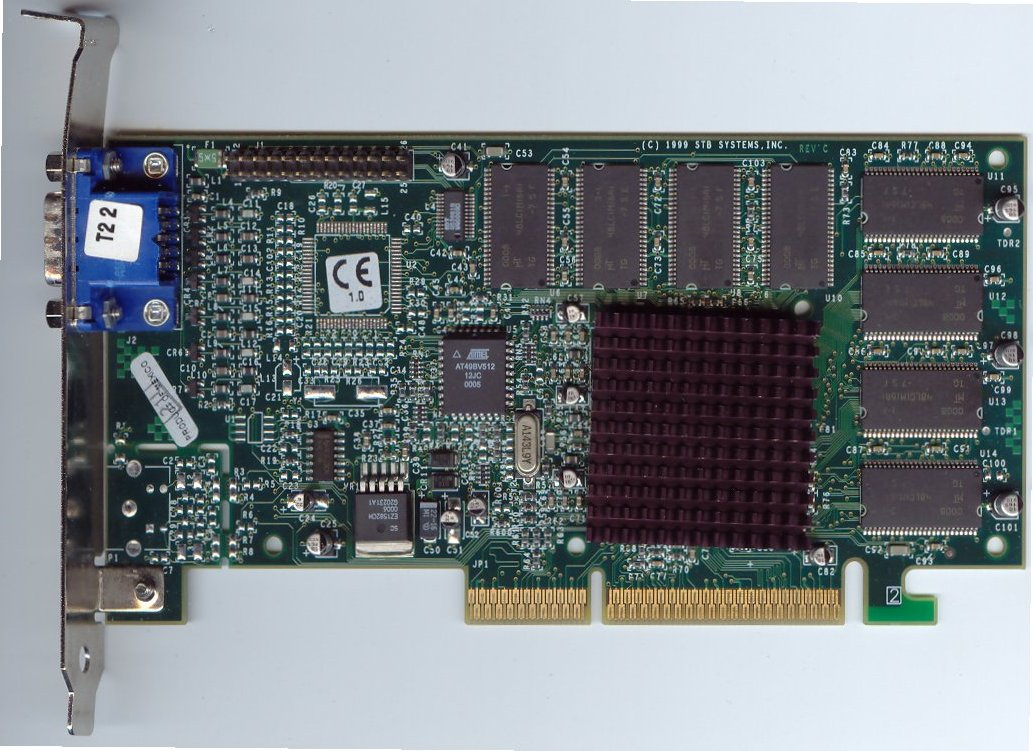
\includegraphics[width=0.8\linewidth]{images/vodoo3.jpg}
        \captionof*{figure}{\scriptsize 3dfx Voodoo 3 - 1999}
        \vspace{0.1cm}
        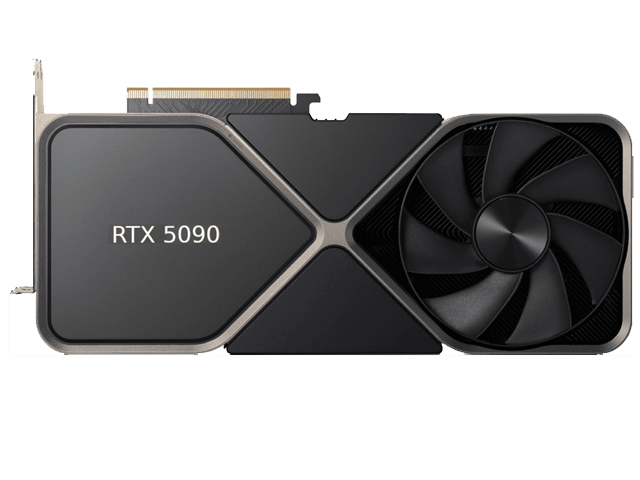
\includegraphics[width=0.8\linewidth]{images/5090.png}
        \vspace*{-0.5cm}
        \captionof*{figure}{\scriptsize NVIDIA GeForce 5090 - 2025}
      \end{center}

      \vspace{1.5cm}

    \end{column}
  \end{columns}
\end{frame}

\subsection{GPU Domination}
\begin{frame}{Why GPUs Dominate Graphics}
  \begin{center}
    \begin{tikzpicture}[scale=0.9]
      % CPU representation
      \node[rectangle, draw, fill=AccentColor!20, minimum width=3cm, minimum height=2cm, align=center] (cpu) at (0,0) {
        \textbf{CPU} \\
        \begin{minipage}{2.8cm}
          \centering
          \scriptsize
          \vspace*{0.2cm}
          4-16 complex cores \\
          Large caches \\
          Branch prediction \\
          Out-of-order execution
        \end{minipage}
      };
      \pause
      % GPU representation
      \node[rectangle, draw, fill=PrimaryColor!20, minimum width=3cm, minimum height=2cm, align=center] (gpu) at (6,0) {
        \textbf{GPU}\\
        \begin{minipage}{2.8cm}
          \centering
          \scriptsize
          \vspace*{0.2cm}
          1000s of simple cores \\
          Small caches \\
          SIMD execution \\
          Throughput optimized
        \end{minipage}
      };
      \pause
      % Task suitability
      \node[below] at (0,-1.35) {
        \begin{minipage}{4cm}
          \centering
          \textcolor{AccentColor}{\textbf{Serial Tasks}} \\
          \scriptsize
          Complex logic \\
          Branching \\
          Low latency
        \end{minipage}
      };
      \pause
      \node[below] at (6,-1.35) {
        \begin{minipage}{4cm}
          \centering
          \textcolor{PrimaryColor}{\textbf{Parallel Tasks}} \\
          \scriptsize
          Simple operations \\
          Same instruction \\
          High throughput
        \end{minipage}
      };
    \end{tikzpicture}
  \end{center}

  \only<5->{
    \begin{raybox}{Perfect Match: Graphics + GPU}
      \textbf{Graphics pipeline stages} process thousands of vertices/fragments \textit{independently} \\
      $\Rightarrow$ Ideal for massively parallel GPU architecture
    \end{raybox}
  }
\end{frame}

\subsection{Modern GPU Architecture}
\begin{frame}{Modern GPU: The Graphics Powerhouse}
  \begin{columns}
    \begin{column}{0.6\textwidth}
      \small
      \begin{conceptbox}{Hardware Implementation}
        \textbf{GPU handles entire pipeline:}
        \begin{itemize}
          \item \textbf{Vertex processing:} Shader cores
          \item \textbf{Rasterization:} Fixed-function units
          \item \textbf{Fragment processing:} Shader cores
          \item \textbf{Memory operations:} ROPs
        \end{itemize}

        \vspace{0.3cm}
        \textbf{GPU Driver handles:}
        \begin{itemize}
          \item Command submission
          \item State management
          \item Resource allocation
        \end{itemize}
      \end{conceptbox}
    \end{column}
    \begin{column}{0.4\textwidth}
      \begin{tikzpicture}[scale=0.7]
        \draw[draw, fill=PrimaryColor!10] (-2.5,-3) rectangle (2.5,1.5);
        \node[above] at (0,1.5) {\textbf{GPU Chip}};

        \foreach \x in {-1.5,-0.5,0.5,1.5} {
          \foreach \y in {0.5,0,-0.5} {
            \node[rectangle, draw, fill=PrimaryColor!40, minimum width=0.5cm, minimum height=0.3cm] at (\x,\y) {};
          }
        }
        \node[left] at (1.2,1.15) {\scriptsize Shader Cores};

        \node[rectangle, draw, fill=SecondaryColor!40, minimum width=3cm, minimum height=0.4cm] (raster) at (0,-1.2) {\scriptsize Rasterizers};
        \node[rectangle, draw, fill=AccentColor!40, minimum width=3cm, minimum height=0.4cm] (rop) at (0,-1.7) {\scriptsize ROPs};
        \node[rectangle, draw, fill=ObjectColor!20, minimum width=3cm, minimum height=0.4cm] (mem) at (0,-2.5) {\scriptsize Video Memory};

        \draw[->, thick] (3,1.3) -- (3,-2.8) node[midway, right] {\scriptsize Pipeline};
      \end{tikzpicture}
    \end{column}
  \end{columns}
\end{frame}
